\documentclass[11pt,a4paper]{article}
\usepackage[margin=2.3cm]{geometry}
\usepackage[T1]{fontenc}
\usepackage{textcomp}
\input{glyphtounicode}
\pdfgentounicode=1
\usepackage{lmodern}
\usepackage{xcolor}
\usepackage{listings}
\usepackage{tcolorbox}
\usepackage{booktabs}
\usepackage{tikz}
\usepackage{hyperref}
\hypersetup{colorlinks=true, linkcolor=blue!50!black, citecolor=green!40!black}

\definecolor{codebg}{RGB}{248,248,245}
\lstset{
  language=C, basicstyle=\ttfamily\footnotesize, backgroundcolor=\color{codebg},
  keywordstyle=\color{blue!60!black}\bfseries, commentstyle=\color{green!45!black}\itshape,
  stringstyle=\color{red!60!black}, numbers=none, upquote=true,
  frame=single, rulecolor=\color{gray!40}, breaklines=true, columns=fullflexible,
  keepspaces=true, showstringspaces=false
}
\lstdefinestyle{sh}{language=bash, backgroundcolor=\color{black!5}}

\newtcolorbox{keyidea}{colback=blue!4, colframe=blue!45!black, title=Key ideas, fonttitle=\bfseries\small}
\newtcolorbox{experiment}{colback=orange!5, colframe=orange!70!black, title=Experiment, fonttitle=\bfseries\small}

\title{\textbf{OpenMP --- Lesson 3}\\[4pt]\large Fixing the race: \texttt{critical}, \texttt{atomic} and \texttt{reduction}}
\author{Study notes for Flor Vargas}
\date{November 2026}

\begin{document}
\maketitle

\noindent\textit{\small Sources: Chapman, Jost \& van der Pas~\cite{chapman}, Ch.~4
``OpenMP Language Features'' (the \texttt{critical} and \texttt{atomic} constructs, the
\texttt{reduction} clause) and Ch.~5 ``How to Get Good Performance'' (cost of
synchronization).}

\section{The idea}
In Lesson~2 several threads incremented a shared \texttt{counter} and increments were
lost. There are two ways to fix it:
\begin{enumerate}
  \item \textbf{Coordinate the threads} so that only one updates the variable at a time:
        \texttt{critical} or \texttt{atomic}. Correct, but threads must wait for each other.
  \item \textbf{Stop sharing}: each thread accumulates into its own private copy, and the
        copies are combined once at the end: \texttt{reduction}. Correct and with no waiting.
\end{enumerate}

\section{The three tools}
\begin{center}
\small
\begin{tabular}{@{}p{4.1cm}p{6.2cm}p{4.9cm}@{}}
\toprule
Tool & What it guarantees & Use it for \\ \midrule
\texttt{\#pragma omp critical} & one thread at a time runs the block (a lock)
  & any code: several statements, calls \\
\texttt{\#pragma omp atomic} & the next single update is indivisible
  & one statement: \texttt{x++}, \texttt{x += e} \\
\texttt{reduction(op:x)} & private copy per thread, combined with \texttt{op} at the end
  & sums, products, max, min \\
\bottomrule
\end{tabular}
\end{center}

\noindent How \texttt{reduction(+:c)} works with 4 threads:
\begin{center}
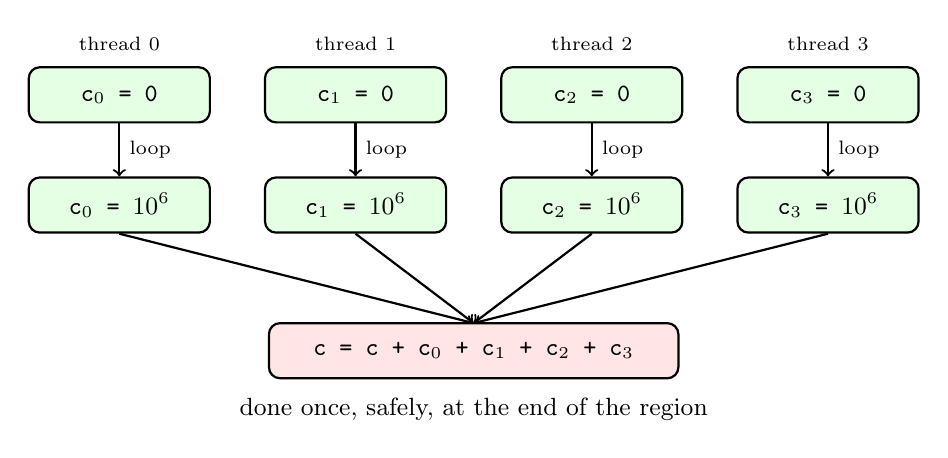
\begin{tikzpicture}[thick, box/.style={draw, rounded corners, minimum width=2.3cm, minimum height=0.7cm, font=\small\ttfamily}]
  \foreach \i/\x in {0/0,1/3,2/6,3/9} {
    \node[box, fill=green!10] (p\i) at (\x,0) {c$_{\i}$ = 0};
    \node[font=\scriptsize] at (\x,0.65) {thread \i};
    \node[box, fill=green!10] (q\i) at (\x,-1.4) {c$_{\i}$ = $10^6$};
    \draw[->] (p\i) -- node[right, font=\scriptsize]{loop} (q\i);
    \draw[->] (q\i.south) -- (4.5,-2.9);
  }
  \node[box, fill=red!10, minimum width=5.2cm] at (4.5,-3.25) {c = c + c$_0$ + c$_1$ + c$_2$ + c$_3$};
  \node[font=\small] at (4.5,-4.0) {done once, safely, at the end of the region};
\end{tikzpicture}
\end{center}
The private copy is initialised to the \emph{identity} of the operator: 0 for \texttt{+},
1 for \texttt{*}.

\section{The code}
The same counter as Lesson~2, written four times: the race, then each fix. Each version
is timed with \texttt{omp\_get\_wtime()}, which returns wall-clock seconds.

\lstinputlisting[title=\texttt{fix\_race.c}]{fix_race.c}

\begin{lstlisting}[style=sh]
gcc -Wall -fopenmp -o fix_race fix_race.c
OMP_NUM_THREADS=4 ./fix_race
\end{lstlisting}
Typical output (your times will differ):
\begin{lstlisting}[style=sh]
threads = 4, expected = 4000000

race      :   2402115   0.0087 s
critical  :   4000000   0.4488 s
atomic    :   4000000   0.1637 s
reduction :   4000000   0.0019 s
\end{lstlisting}

\begin{keyidea}
\begin{itemize}
  \item All three fixes give the correct result. They differ only in cost.
  \item \texttt{critical} is the most general and the most expensive: every increment
        takes and releases a lock, and the other threads wait.
  \item \texttt{atomic} is cheaper because the hardware does the update in one
        indivisible instruction, but it still forces threads to take turns on one
        memory location.
  \item \texttt{reduction} has no synchronization inside the loop. It is the right tool
        whenever the pattern is ``combine many values with one operator''.
  \item Rule of thumb: prefer \texttt{reduction} $>$ \texttt{atomic} $>$ \texttt{critical}.
\end{itemize}
\end{keyidea}

\section{The experiment}
\begin{experiment}
\textbf{Question:} how does the cost of each fix change as the number of threads grows?
\begin{enumerate}
  \item Run with 1, 2 and 4 threads:
\begin{lstlisting}[style=sh]
for t in 1 2 4; do echo "== $t threads"; OMP_NUM_THREADS=$t ./fix_race; done
\end{lstlisting}
  \item Write the times in a table: rows = method, columns = number of threads.
\end{enumerate}
\textbf{What to observe and answer.}
\begin{enumerate}
  \item With 1 thread, \texttt{critical} and \texttt{atomic} are already slower than
        \texttt{reduction}, although there is nobody to wait for. Why?
  \item As threads are added, the work per thread stays the same but \texttt{critical}
        and \texttt{atomic} get \emph{slower}. Why does adding threads make them worse?
  \item Why does \texttt{reduction} stay fast?
\end{enumerate}
\end{experiment}

\paragraph{Answers (read after trying).}
(1)~Synchronization has a fixed cost even with no competition: taking and releasing a
lock, or executing a locked hardware instruction, is much slower than a plain
\texttt{c++}. We pay it $10^6$ times.
(2)~More threads means more of them competing for the same lock or memory location
(\emph{contention}). The updates are forced into a single line, so the program runs
essentially serially, plus the overhead of handing the variable from one core to another.
(3)~Each thread works only on its private copy, so the threads never wait for each other.
The single combining step at the end costs almost nothing. Lesson: the fastest
synchronization is the one you avoid.

\paragraph{Next lesson.} Sharing the \emph{work}: so far every thread did all $N$
iterations. The \texttt{for} work-sharing construct splits one loop's iterations among
the threads (Chapman et al., Ch.~4).

\begin{thebibliography}{9}
\bibitem{chapman} B.~Chapman, G.~Jost, and R.~van der Pas. \emph{Using OpenMP: Portable
  Shared Memory Parallel Programming}. MIT Press, Cambridge, MA, 2007.
\end{thebibliography}
\end{document}
